
\subsection{Code Deployment \& Image Building}
\begin{figure}[H]
    \centering
    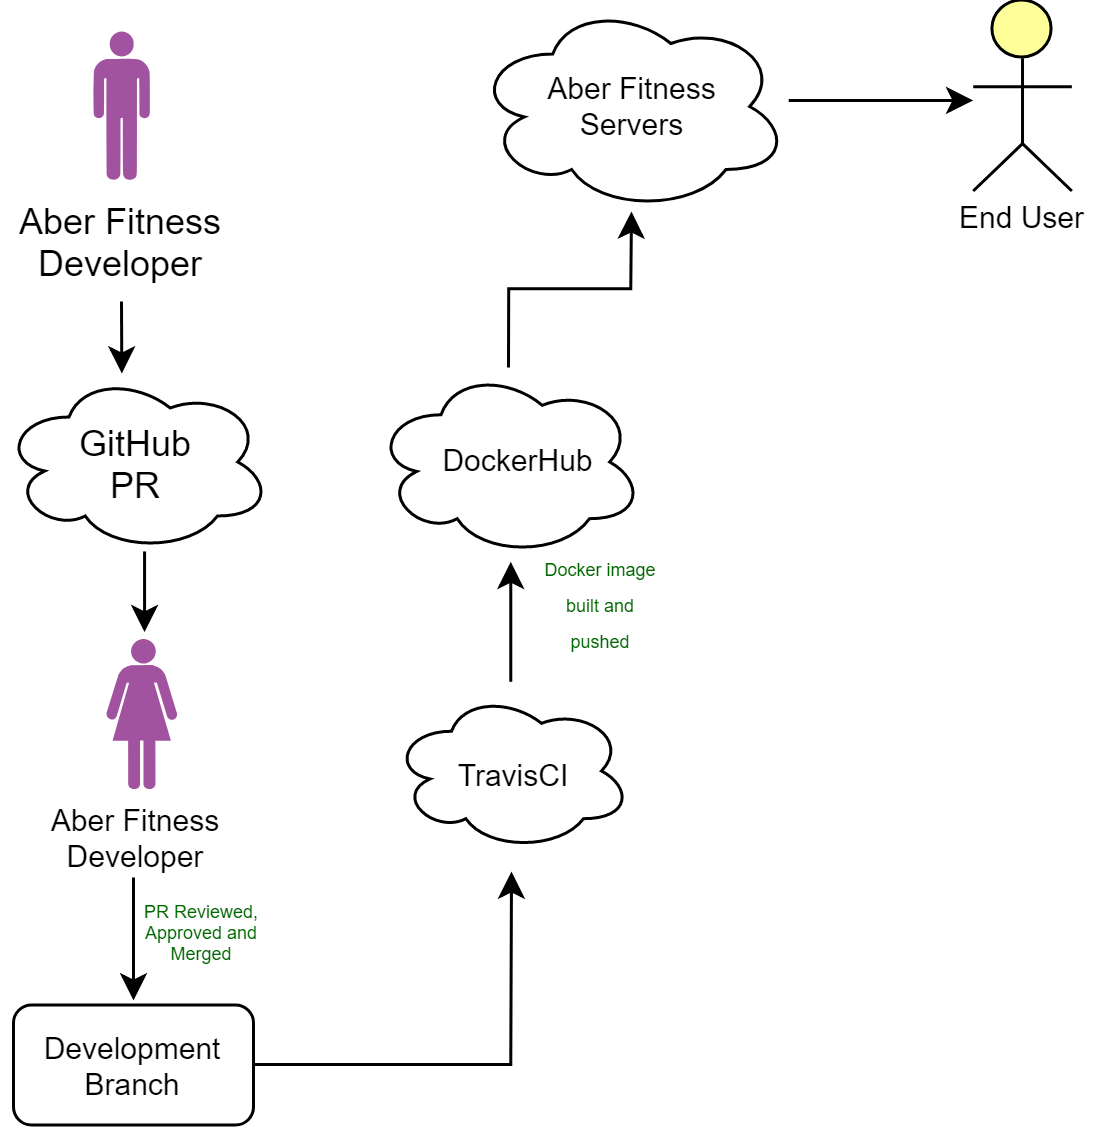
\includegraphics[width=0.8\textwidth]{Images/diagram_af.png}
    \caption{Aber Fitness development process flow diagram}
\end{figure}

The above diagram (\textbf{TODO: link fig ref}) outlines our deployment and code review process. After a pull request had been reviewed by another member of the team and Travis CI had built the application to ensure that all unit tests pass, the pull request would then be merged into the \lstinline{development} branch. Any pushes to the \lstinline{development} branch would trigger Travis CI to then run a script within the application repository, \lstinline{bin/docker.sh}. This script was responsible for building the application into a Docker image and pushing it up to Docker Hub. Once the image had been built and pushed, the application was then ready for deployment to our staging host, \textit{docker2.aberfitness.biz}, the developer could then issue the \lstinline{/deploy} command within Slack to begin the re-deployment of our entire Docker stack\footnote{A 'stack' is a collection of Docker images grouped together through a \textbf{docker-compose.yml} file}. \textbf{TODO: clarify this}

This deployment flow typically worked very well for us throughout the development process, allowing us to easily deploy code updates to \textit{docker2.aberfitness.biz} while also ensuring that code had been peer reviewed and unit tested before being rolled out onto a live server. Our deployment flow relied heavily upon GitHub and Travis, as they were responsible for hosting our code and generating Docker images respectively. While the majority of the time these services worked out incredibly well for us, we had a few issues during incidents where TravisCI was suffering from outages, rendering us unable to deploy code updates, adding a few delays to the development process.

\subsubsection{nginx, MariaDB, Syslog}
\begin{figure}[H]
    \centering
    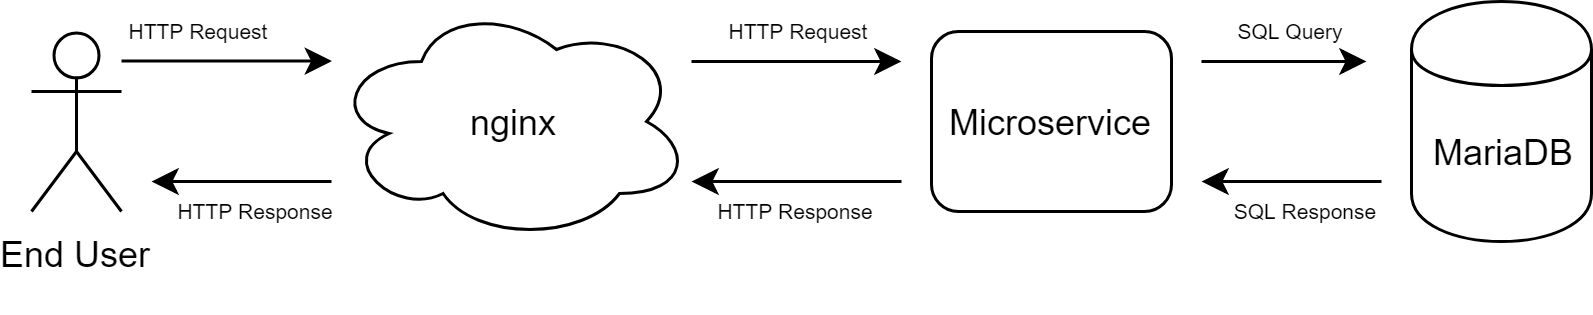
\includegraphics[width=\textwidth]{Images/nginx_proxy_flow.png}
    \caption{Traffic flow diagram showing an end user's browser connecting to the internet facing \textit{nginx} server, which then proxies requests through to the backend microservice}
\end{figure}

